\section{Introducción}
La planificación de la producción es una disciplina clave en la gestión de 
activos y se utiliza para determinar la forma más eficiente de asignar 
recursos, como maquinaria, mano de obra y tiempo, con el fin de alcanzar 
los objetivos de producción. Es un proceso que implica la toma de decisiones 
sobre qué recursos, cuánto, cuándo y cómo producirlos, con el objetivo de optimizar la 
utilización de los elementos disponibles, maximizando la eficiencia y rentabilidad 
del proceso de producción. La planificación de la producción se aplica en una 
amplia gama de sectores y áreas de negocio, incluyendo la fabricación, la logística, 
el transporte, la distribución y la gestión de la cadena de suministro, entre otros.\medskip

La importancia de la planificación de la producción radica en su capacidad para mejorar 
la eficiencia mediante una buena gestión de las operaciones, lo que puede tener un impacto 
significativo en la rentabilidad y competitividad de las empresas. Una planificación de 
producción efectiva debe optimizar la asignación de recursos, minimizar los tiempos de 
inactividad, reducir los costos de producción y maximizar el cumplimiento de los plazos 
de entrega en la medida de lo posible. Esto lo que resulta es en una mayor eficiencia operativa 
y una mejor calidad del producto o servicio.\medskip

Sin embargo, la planificación de la producción es un problema complejo debido a la gran 
cantidad de variables y restricciones que deben tenerse en cuenta, como los tiempos de 
procesamiento, las capacidades de los recursos, las restricciones de almacenamiento y 
transporte y las demandas de los clientes, entre otros. Tradicionalmente, este problema 
se ha abordado utilizando enfoques heurísticos y meta-heurísticos como el 
Job Shop Scheduling Problem (JSP) y el Flexible Shop Scheduling Problem (FJSP), que son problemas 
combinatorios y conocidos por ser NP-Hard, lo que implica que no existen algoritmos eficientes 
para encontrar soluciones óptimas en un tiempo razonable.\medskip

Un problema NP-Hard es un tipo de problema de optimización en el cual no se conocen algoritmos 
exactos que puedan encontrar una solución óptima en un tiempo polinómico. Esto implica que a 
medida que el tamaño del problema aumenta, el tiempo de cómputo necesario para encontrar una 
solución óptima también se vuelve prohibitivamente alto. Estos problemas son considerados de 
gran complejidad y representan un desafío significativo para la investigación en ciencias de 
la computación. La importancia de identificar un problema como NP-Hard radica en que a menudo 
tecnicas utilizadas para un problema pueden ser aplicados a otros problemas NP-Hard. Esto se debe a que 
muchos problemas NP-Hard comparten estructuras y patrones similares, lo que permite la 
transferencia de conocimientos y técnicas de un problema a otro. Por lo tanto, encontrar 
soluciones eficientes o aproximadas para un problema NP-Hard particular puede tener un impacto 
significativo en la resolución de otros problemas que enfrentan desafíos similares.\medskip

En los últimos años, ha surgido el Imitation Learning como una prometedora técnica de aprendizaje 
automático. El Imitation Learning se basa en el concepto de aprender de la experiencia de expertos 
humanos o de sistemas previamente establecidos, y luego utilizar ese conocimiento para 
guiar la toma de decisiones en situaciones similares. Esto se puede lograr a través de enfoques 
supervisados, donde se entrena a un modelo para imitar las acciones de expertos humanos, o 
a través de enfoques de Reinforcement Learning (RL), donde se permite que un modelo aprenda a 
partir de la retroalimentación y la interacción con el entorno.\medskip

En este contexto, el presente trabajo se enfoca en el desarrollo de un sistema de planificación 
basado en Imitation Learning, utilizando técnicas de aprendizaje supervisado y RL para resolver el FJSP. 
Se busca explorar cómo estas técnicas pueden aplicarse a la planificación de la producción, teniendo 
en cuenta los desafíos y la complejidad de este problema. A través del estudio y análisis de 
diferentes enfoques y metodologías, se pretende contribuir al campo de la planificación de la 
producción utilizando técnicas de inteligencia artificial y aprendizaje automático, con el objetivo 
de mejorar la eficiencia y la toma de decisiones en procesos industriales.\medskip

\subsection{Motivación}
La planificación de la producción es un desafío constante en la industria, ya que puede tener 
un impacto significativo en la eficiencia, la productividad y la rentabilidad de las operaciones 
de fabricación. Sin embargo, muchos de los problemas de planificación de la producción en la 
industria, como el Job Shop Scheduling Problem (JSP) y el Flexible Job Shop Scheduling Problem (FJSP), 
son conocidos por su alta complejidad y la falta de soluciones eficientes. Esto puede resultar 
en cuellos de botella, retrasos en la producción y costos innecesarios.\medskip

Es crucial encontrar soluciones innovadoras y eficientes que puedan abordar 
los desafíos complejos asociados con la planificación de la producción en entornos que enfrentan 
problemas NP-Hard. Además, la aplicación de enfoques de inteligencia artificial y aprendizaje 
automático en la planificación de la producción ha ganado cada vez más atención en la industria 
debido a su potencial para encontrar soluciones aproximadas en tiempo real y adaptarse a 
entornos dinámicos.\medskip

La motivación de este proyecto radica en la necesidad de desarrollar enfoques de Imitation 
Learning, una rama del aprendizaje automático que se basa en la imitación de comportamientos 
de expertos, para abordar los desafíos de la planificación de la producción en la industria. 
Estos enfoques tienen el potencial de mejorar la eficiencia y la productividad de las operaciones 
de fabricación al encontrar soluciones eficientes y adaptativas en tiempo real. Además, las 
soluciones desarrolladas en el contexto del JSP y el FJSP podrían tener aplicaciones amplias 
en otros problemas NP-Hard que enfrenta la industria, como la logística, la programación de 
tareas o la asignación de recursos, lo que podría tener un impacto significativo en la 
optimización de procesos y la competitividad de las empresas en la industria.

\subsection{Explicación del problema}
El Flexible job shop scheduling problem , es un desafío de optimización combinatoria 
que se encuentra en el campo de la la gestión de la producción. En este problema, se busca determinar 
la secuencia óptima de operaciones a realizar en una serie de máquinas, con el objetivo de minimizar el 
tiempo total de producción o maximizar la eficiencia del sistema. A diferencia del Job shop scheduling 
problem, en el que cada operación tiene una ruta de procesamiento fija, las operaciones pueden ser 
procesadas en varias máquinas diferentes. Además, adicionalmente las operaciones estan agrupadas 
dentro de un trabajo, que es un conjunto de operaciones que deben ser procesadas en una secuencia
específica.\medskip

Existen dos restricción temporales que especifican cuándo puede comenzar 
cada operación: una operación no puede comenzar hasta que se hayan completado todas las operaciones
anteriores de la misma tarea y no puede comenzar hasta que se hayan completado todas las operaciones
anteriores de la misma máquina. El objetivo del problema es asignar las operaciones a las máquinas y determinar el orden de procesamiento 
del sistema manera óptima, teniendo en cuenta las restricciones temporales y los recursos disponibles, 
de manera que se minimice el tiempo total de producción. El tiempo total de producción se refiere al
tiempo de finalización de la máquina más lenta, que se calcula sumando el tiempo de procesamiento 
de todas las operaciones y el gap que estas generan.\medskip

Para ilustrar el problema, supongamos que tenemos una fabrica que produce tres tipos de productos
que se definen como los trabajos: A, B y C. Contamos con tres máquinas: M1, M2, M3 y M4 
y cada producto requiere hacer ciertas operaciones de procesamiento en estas máquinas en 
un orden específico. Las operaciones y los tiempos de procesamiento estimados para cada 
producto en cada máquina son los siguientes: 

\begin{table}[ht]
    \caption{Tiempos de procesamiento estimados para cada producto} 
    \centering 
    \begin{tabular}{ccccccccc}  

    \toprule
    \multirow{2}{*}{\parbox[c]{.2\linewidth}{\centering Maquina ID}} & 
    \multicolumn{2}{c}{Trabajo A} && 
    \multicolumn{2}{c}{Trabajo B} && 
    \multicolumn{2}{c}{Trabajo C} \\ 

    \cmidrule{2-3} \cmidrule{5-6} \cmidrule{8-9}
     & {\centering OP 1} & {OP 2} && {OP 3} & {OP 4} && {OP 5}\\

    \midrule
    Máquina 1 & 4 UT & --   && 3 UT & 7 UT && 1 UT & -- \\
    Máquina 2 & 3 UT & 2 UT && 2 UT & 2 UT && 6 UT & -- \\
    Máquina 3 & 2 UT & 1 UT && --   & 5 UT && 2 UT & -- \\  
    Máquina 4 & --   & 3 UT && 4 UT & 8 UT && 3 UT & -- \\ 
    \bottomrule
    
    \end{tabular}
\end{table}

\medskip

Aquí, cada operación se identifica con un número y el tipo de procesamiento se mide en Unidades temporales
(UD). Las operaciones que no se pueden realizar en una máquina se identifican con un guión (-), lo que 
significa que en este ejemplo la máquina 1 podría procesar las operaciones 1, 3, 4 y 5 pero 
no la operación 2. Una vez entendida la distribución de tiempos de procesamiento, podemos visualizar
el resultado de la planificación en el siguiente diagrama, donde cada caja representa una operación 
y cada línea representa una máquina.

\begin{figure}[ht]
    \centering
    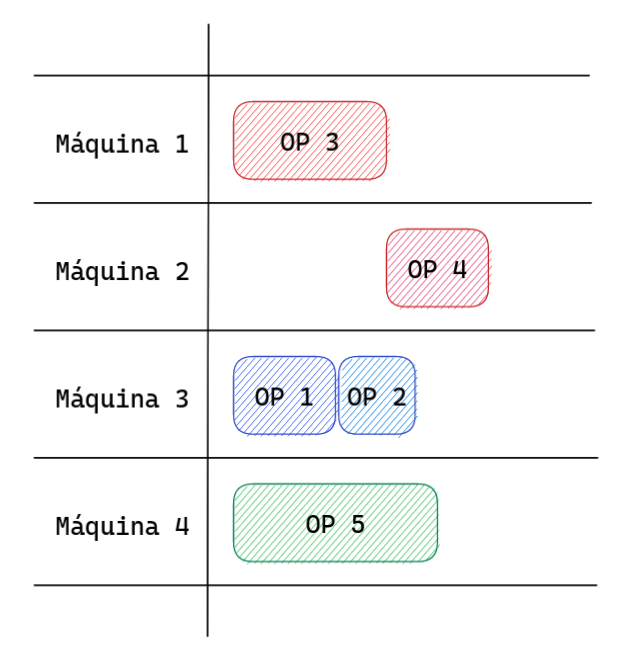
\includegraphics[scale=0.40]{ejemplo.png}
    \caption{Ejemplo de planificación óptima}
    \label{fig:example-solution}
\end{figure}

La distribución final de tiempos para cada máquina es la siguiente: 
\begin{itemize}
    \item \textbf{maquina 1}, OP 3 (3 UT) + 0 GAP = 3 UT 
    \item \textbf{maquina 2}, OP 4 (2 UT) + 3 GAP = 5 UT 
    \item \textbf{maquina 3}, OP 1 (2 UT) + OP 2 (1 UT) + 0 GAP = 3 UT 
    \item \textbf{maquina 4}, OP 5 (4 UT) + 0 GAP = 4 UT. 
\end{itemize}

Ya que el tiempo total de producción es el tiempo de finalización de la máquina más lenta, 
que es la máquina 2, son 5 UT. Notese que el gap de la máquina 2 es deribado de la dependencia
existente entre la operación 4 y la operación 3 por petenercer ambos al trabajo B, 
por lo tanto, antes de que dicha maquina empiece con la operacion 4 tiene que esperar 
a que se procese la máquina 1.

\subsection{Estructura del documento}



\pagebreak